\chapter{翻译的限度}
\label{ch:01}

\begin{chapterquote}{——示例题词，\textit{An Essay on Translation}}
翻译不是把一种语言换成另一种语言，而是让另一种语言里的经验，在中文里重新变得可理解。
\end{chapterquote}

\section{两种忠实}

把 \term{忠实}{fidelity} 理解为逐字对应，是翻译讨论中最常见的误会。词与词之间并不存在稳定的等号：一个英文词的含义，取决于它在句中的位置、它与前后词的搭配，以及它所处时代的用法。译者若只盯着词，得到的往往是一串语法正确、意义悬空的句子。

更可行的做法，是把忠实分成两层。第一层是\textbf{信息}的忠实：谁做了什么、在什么时候、对谁、带着什么限定。第二层是\textbf{语气}的忠实：作者是在陈述、在讽刺、在迟疑，还是在替读者预先反驳。第一层可以靠对照检查；第二层只能靠反复读原文，读出那些没有写出来的东西。\zhu{“没有写出来的东西”指预设、反讽与情感色彩，不是指原文省略的信息；译者不得据此补写正文。}

这两层并不总是同时满足。中文的句法偏好短句与意合，英文的论证却常用长句与形合；把长句拆开，信息仍在，语气却可能变硬。\zhu{这是句法重组的典型代价。处理办法是保留逻辑连接词或调整语序，而不是删除限定语。}反过来，为了保留语气而照搬英文句法，中文读者又会被层层嵌套的从句挡住。译者的工作，是在两者之间找一个具体段落、具体读者能够接受的平衡点，而不是宣布一条普遍原则。

\section{一个例子}

下面这段英文讨论译者在两种语言之间的位置：

\begin{quote}
A translator works at the edge of two languages: close enough to hear the rhythm of the original, far enough to know what a reader of the target language will not hear.
\end{quote}

直译可以成立：“译者在两种语言的边缘工作：近得足以听见原文的节奏，远得足以知道目标语读者听不见什么。”信息是完整的，但“边缘”“近得”“远得”三个空间隐喻在中文里略显生硬。若改成“译者站在两种语言之间：既要贴近原文的节奏，又要清楚中文读者会漏掉什么”，读起来更顺，却把原文的对称结构改成了让步关系。两种译法各有代价，选择哪一种，取决于这本书整体上是学术专著还是普及读物。

\begin{figure}[htbp]
  \centering
  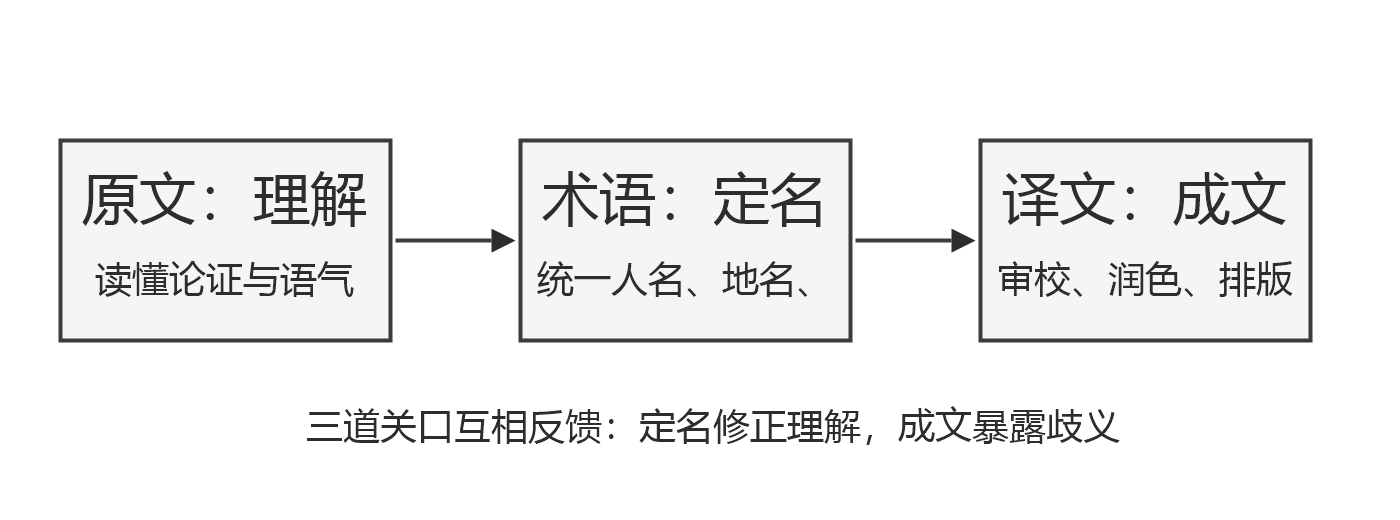
\includegraphics[width=0.72\textwidth]{figures/fig1-1.png}
  \caption{翻译流程中的三道关口：理解、定名、成文。}
  \label{fig:translation-gates}
  \figsource{示意图，由工作区模板生成。}
\end{figure}

如图 \ref{fig:translation-gates} 所示，三道关口并非线性通过：定名会反过来修正理解，成文又会暴露此前未察觉的歧义。因此，初译、审校、润色必须分开进行，不能指望一遍完成。

\section{术语与注释}

术语的一致性不是排版问题，而是理解问题。同一原文词在不同章节被译成不同中文，通常说明译者对该词的理解尚未稳定；反过来，强行统一一个多义词，也会让译文在某个语境里失真。可行的做法是：在 \texttt{glossary/terms.csv} 中记录定名、语境与禁用变体，由脚本在全书范围检查，而不是靠记忆。

原书脚注必须全部译出。脚注往往不是装饰，而是作者与同行对话的痕迹；删掉脚注，等于删掉论证的一部分。\footnote{示例原注：此处模拟原书脚注的排印方式，编号与正文对应。}译者注则用来处理另一种情况：原文的预设对中文读者不成立，或双关无法保留。两者都出现在页脚，但文本上必须可区分。

\begin{table}[htbp]
  \centering
  \caption{三类注释的处理方式}
  \label{tab:notes}
  \begin{tabular}{@{}lll@{}}
    \toprule
    类型 & 标记 & 处理原则 \\
    \midrule
    原书脚注 & \texttt{\textbackslash footnote} & 全译，不改编号关系 \\
    译者注 & \texttt{\textbackslash zhu} & 说明背景、双关、译名理由 \\
    原文夹注 & 括号 & 原样保留，不改成脚注 \\
    \bottomrule
  \end{tabular}
\end{table}

翻译的限度，说到底不是语言的限度，而是译者愿意在多大程度上贴近原文、又愿意在多大程度上为读者负责。这两件事并不矛盾；矛盾的是以为可以只做其中一件。
